\documentclass[12pt]{beamer}
\usepackage{../Estilos/BeamerFC}
\usepackage{../Estilos/ColoresLatex}
\usepackage{courier}
\usepackage{listingsutf8}
\usepackage{listings}
\usepackage{xcolor}
\usepackage{textcomp}
\usepackage{color}
\definecolor{deepblue}{rgb}{0,0,0.5}
\definecolor{brown}{rgb}{0.59, 0.29, 0.0}
\definecolor{OliveGreen}{rgb}{0,0.25,0}
% \usepackage{minted}

\DeclareCaptionFont{white}{\color{white}}
\DeclareCaptionFormat{listing}{\colorbox{gray}{\parbox{0.98\textwidth}{#1#2#3}}}
\captionsetup[lstlisting]{format=listing,labelfont=white,textfont=white}
\renewcommand{\lstlistingname}{Código}


\definecolor{Code}{rgb}{0,0,0}
\definecolor{Keywords}{rgb}{255,0,0}
\definecolor{Strings}{rgb}{255,0,255}
\definecolor{Comments}{rgb}{0,0,255}
\definecolor{Numbers}{rgb}{255,128,0}

\makeatletter

\newif\iffirstchar\firstchartrue
\newif\ifstartedbyadigit
\newif\ifprecededbyequalsign

\newcommand\processletter
{%
  \ifnum\lst@mode=\lst@Pmode%
    \iffirstchar%
        \global\startedbyadigitfalse%
      \fi
      \global\firstcharfalse%
    \fi
}

\newcommand\processdigit
{%
  \ifnum\lst@mode=\lst@Pmode%
      \iffirstchar%
        \global\startedbyadigittrue%
      \fi
      \global\firstcharfalse%
  \fi
}

\lst@AddToHook{OutputOther}%
{%
  \lst@IfLastOtherOneOf{=}
    {\global\precededbyequalsigntrue}
    {}%
}

\lst@AddToHook{Output}%
{%
  \ifprecededbyequalsign%
      \ifstartedbyadigit%
        \def\lst@thestyle{\color{orange}}%
      \fi
    \fi
  \global\firstchartrue%
  \global\startedbyadigitfalse%
  \global\precededbyequalsignfalse%
}

\lstset{ 
language=Python,                % choose the language of the code
basicstyle=\footnotesize\ttfamily,       % the size of the fonts that are used for the code
numbers=left,                   % where to put the line-numbers
numberstyle=\scriptsize,      % the size of the fonts that are used for the line-numbers
stepnumber=1,                   % the step between two line-numbers. If it is 1 each line will be numbered
numbersep=5pt,                  % how far the line-numbers are from the code
backgroundcolor=\color{white},  % choose the background color. You must add \usepackage{color}
showspaces=false,               % show spaces adding particular underscores
showstringspaces=false,         % underline spaces within strings
showtabs=false,                 % show tabs within strings adding particular underscores
frame=single,   		% adds a frame around the code
tabsize=2,  		% sets default tabsize to 2 spaces
captionpos=t,   		% sets the caption-position to bottom
breaklines=true,    	% sets automatic line breaking
breakatwhitespace=false,    % sets if automatic breaks should only happen at whitespace
escapeinside={| |},  % if you want to add a comment within your code
stringstyle =\color{OliveGreen},
otherkeywords={as, np.array, np.concatenate, np.linspace, linspace, interpolate.interp1d, kind, plt.plot, .copy, np.arange, np.cos, np.pi, lw, ls, label, splrep, splev, plt.legend, loc, plt.title, plt.ylim, plt.show, sign, math.ceil, math.log, np.sqrt, np.exp, np.zeros, plt.xlabel, plt.ylabel, plt.xlim, np.identity, random, np.dot, np.outer, np.diagonal },             % Add keywords here
keywordstyle = \color{blue},
commentstyle = \color{darkcerulean},
identifierstyle = \color{black},
literate=%
         {á}{{\'a}}1
         {é}{{\'e}}1
         {í}{{\'i}}1
         {ó}{{\'o}}1
         {ú}{{\'u}}1
%
%keywordstyle=\ttb\color{deepblue}
%fancyvrb = true,
}

\lstdefinestyle{FormattedNumber}{%
    literate={0}{{\textcolor{red}{0}}}{1}%
             {1}{{\textcolor{red}{1}}}{1}%
             {2}{{\textcolor{red}{2}}}{1}%
             {3}{{\textcolor{red}{3}}}{1}%
             {4}{{\textcolor{red}{4}}}{1}%
             {5}{{\textcolor{red}{5}}}{1}%
             {6}{{\textcolor{red}{6}}}{1}%
             {7}{{\textcolor{red}{7}}}{1}%
             {8}{{\textcolor{red}{8}}}{1}%
             {9}{{\textcolor{red}{9}}}{1}%
             {.0}{{\textcolor{red}{.0}}}{2}% Following is to ensure that only periods
             {.1}{{\textcolor{red}{.1}}}{2}% followed by a digit are changed.
             {.2}{{\textcolor{red}{.2}}}{2}%
             {.3}{{\textcolor{red}{.3}}}{2}%
             {.4}{{\textcolor{red}{.4}}}{2}%
             {.5}{{\textcolor{red}{.5}}}{2}%
             {.6}{{\textcolor{red}{.6}}}{2}%
             {.7}{{\textcolor{red}{.7}}}{2}%
             {.8}{{\textcolor{red}{.8}}}{2}%
             {.9}{{\textcolor{red}{.9}}}{2}%
             {\ }{{ }}{1}% handle the space
         ,%
          %mathescape=true
          escapeinside={__}
          }



\usetheme{Warsaw}
\usecolortheme{seahorse}
%\useoutertheme{default}
\setbeamercovered{invisible}
% or whatever (possibly just delete it)
\setbeamertemplate{section in toc}[sections numbered]
\setbeamertemplate{subsection in toc}[subsections numbered]
\setbeamertemplate{subsection in toc}{\leavevmode\leftskip=3.2em\rlap{\hskip-2em\inserttocsectionnumber.\inserttocsubsectionnumber}\inserttocsubsection\par}
\setbeamercolor{section in toc}{fg=blue}
\setbeamercolor{subsection in toc}{fg=blue}
\setbeamercolor{frametitle}{fg=blue}
\setbeamertemplate{caption}[numbered]

\setbeamertemplate{footline}
\beamertemplatenavigationsymbolsempty
\setbeamertemplate{headline}{}


\makeatletter
\setbeamercolor{section in foot}{bg=gray!30, fg=black!90!orange}
\setbeamercolor{subsection in foot}{bg=blue!30}
\setbeamercolor{date in foot}{bg=black}
\setbeamertemplate{footline}
{
  \leavevmode%
  \hbox{%
  \begin{beamercolorbox}[wd=.333333\paperwidth,ht=2.25ex,dp=1ex,center]{section in foot}%
    \usebeamerfont{section in foot} \insertsection
  \end{beamercolorbox}%
  \begin{beamercolorbox}[wd=.333333\paperwidth,ht=2.25ex,dp=1ex,center]{subsection in foot}%
    \usebeamerfont{subsection in foot}  \insertsubsection
  \end{beamercolorbox}%
  \begin{beamercolorbox}[wd=.333333\paperwidth,ht=2.25ex,dp=1ex,right]{date in head/foot}%
    \usebeamerfont{date in head/foot} \insertshortdate{} \hspace*{2em}
    \insertframenumber{} / \inserttotalframenumber \hspace*{2ex} 
  \end{beamercolorbox}}%
  \vskip0pt%
}
\makeatother

\makeatletter
\patchcmd{\beamer@sectionintoc}{\vskip1.5em}{\vskip0.8em}{}{}
\makeatother

%\newlength{\depthofsumsign}
%\setlength{\depthofsumsign}{\depthof{$\sum$}}
% \newcommand{\nsum}[1][1.4]{% only for \displaystyle
%     \mathop{%
%         \raisebox
%             {-#1\depthofsumsign+1\depthofsumsign}
%             {\scalebox
%                 {#1}
%                 {$\displaystyle\sum$}%
%             }
%     }
% }
\def\scaleint#1{\vcenter{\hbox{\scaleto[3ex]{\displaystyle\int}{#1}}}}
\def\scaleoint#1{\vcenter{\hbox{\scaleto[3ex]{\displaystyle\oint}{#1}}}}
\def\bs{\mkern-12mu}

\usefonttheme{serif}

\title{\large{Tema 1 - Errores y artimética de punto flotante}}
\author{M. en C. Gustavo Contreras Mayén}
\date{ }

\begin{document}
\maketitle

\section*{Contenido}
\frame[allowframebreaks]{\frametitle{Contenido} \tableofcontents[currentsection, hideallsubsections]}

\section{Más conceptos importantes}
\frame{\tableofcontents[currentsection, hideothersubsections]}
\subsection{Condición}

\begin{frame}
\frametitle{Condición}
La condición (\emph{condicionamiento}) de una función $f(x)$ mide la sensibilidad de los valores de $f(x)$ a pequeños
cambios de $x$, se define como:
\pause
\begin{align*}
C = \abs{ \dfrac{E_{\text{rel}} \, (f (x))}{E_{_\text{rel}} (x)} }
\end{align*}
\end{frame}
\begin{frame}
\frametitle{Definición de condición}
Del teorema del valor medio en cálculo, podemos expresar:
\pause
\begin{eqnarray*}
\begin{aligned}
f (x_{T}) - f (x_{A})  &\approx \pderivada{f} (x_{T}) \, (x_{T} - x_{A}) \\ \pause
\rightarrow E_{\text{rel}} (f (x)) &\approx \dfrac{ \pderivada{f} (x_{T})}{ f(x_{T})} (x_{T} - x_{A})
\end{aligned}
\end{eqnarray*}
luego entonces:
\pause
\begin{align*}
C \approx \abs{ x_{T} \dfrac{\pderivada{f} (x_{T})}{f (x_{T})} }
\end{align*}
\end{frame}
\begin{frame}
\frametitle{Definición de condición}
Se utilizará a $C$ como definición de condición para funciones $f (x)$ de una variable real.
\\
\bigskip
\pause
Entonces el número de condición será:
\pause
\begin{align*}
C = \abs{ x \, \dfrac{\pderivada{f} (x)}{f (x)} }
\end{align*}
\end{frame}
\begin{frame}
\frametitle{Valores del número de condición}
\setbeamercolor{item projected}{bg=red,fg=white}
\setbeamertemplate{enumerate items}{%
\usebeamercolor[bg]{item projected}%
\raisebox{1.5pt}{\colorbox{bg}{\color{fg}\footnotesize\insertenumlabel}}%
}
\begin{enumerate}[<+->]
\item Para un $x$ dado $0 < C (x) < 1$ se dirá que \emph{el problema está bien condicionado}, \pause y cuanto menor sea $C$, mejor condicionado. \pause
\item Si $C (x) > 1$, el problema estará mal condicionado.
\item Si $C (x) = 1$, el error relativo se mantiene.
\end{enumerate}
\end{frame}
\begin{frame}
\frametitle{Ejemplos}
¿Las siguientes funciones están bien condicionadas?
\pause
\setbeamercolor{item projected}{bg=cadetblue,fg=amber}
\setbeamertemplate{enumerate items}{%
\usebeamercolor[bg]{item projected}%
\raisebox{1.5pt}{\colorbox{bg}{\color{fg}\footnotesize\insertenumlabel}}%
}
\begin{enumerate}[<+->]
\item $f (x) = \sqrt{x} \hspace{1.5cm} C (x) = ?$
\item $g (x) = x^{2} - 1 \hspace{1.5cm} C (x) = ?$
\end{enumerate}
\end{frame}
\begin{frame}
\frametitle{Los números de condición}
Haciendo las cuentas tendremos que para las funciones:
\pause
\begin{align*}
C (f (x) ) = \dfrac{1}{2} \hspace{0.75cm} &\Rightarrow 0 < C (f (x) ) < 1 \\
\therefore \quad &\text{Problema bien condicionado}
\end{align*}
\end{frame}
\begin{frame}
\frametitle{Los números de condición}
El $C (g (x) )$ lo visualizamos con una gráfica:
\pause
\begin{figure}
	\centering
	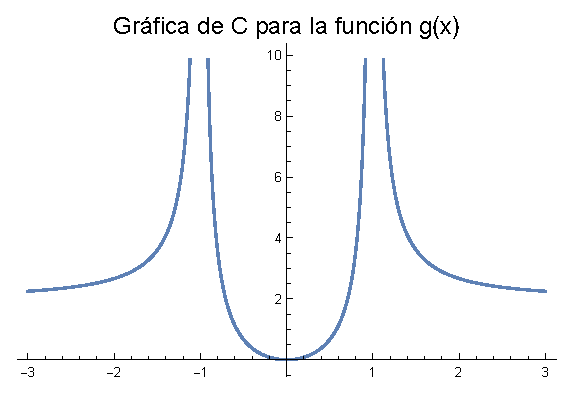
\includegraphics[scale=0.85]{Imagenes/Condicion_02.eps}
\end{figure}
\end{frame}

\section{Polinomios de Taylor}
\frame{\tableofcontents[currentsection, hideothersubsections]}
\subsection{Su uso en cómputo}


\begin{frame}
\frametitle{Los polinomios de Taylor}
\begin{itemize}[<+->]
\item[\ding{212}] Las soluciones numéricas son en su mayoría, aproximaciones de las soluciones exactas.
\item[\ding{212}] Gran parte de los métodos numéricos se basan en la aproximación de funciones por medio de polinomios.
\end{itemize}
\end{frame}
\begin{frame}
\frametitle{Los polinomios de Taylor}
Estos polinomios de Taylor se ocupan para aproximar funciones trascendentes para las cuales no existe una expresión explícita calculable en una cantidad finita de pasos.
\\
\bigskip
\pause
Tales como: \pause aquéllas con radicales o funciones trigonométricas.
\end{frame}
\begin{frame}
\frametitle{Otros polinomios}
De la matemática conocemos otros tipos de polinomios: \pause \textit{de las funciones especiales}: Chebyshev, Legendre, Laguerre, Hermite, etc.
\\
\bigskip
\pause
Preo los polinomios de Taylor son los más utilizados.
\end{frame}
\begin{frame}
\frametitle{Los polinomios de Taylor}
El polinomio de Taylor es una serie infinita de potencias que representa de manera \enquote{exacta} a una función dentro de un cierto radio alrededor de un punto dado.
\\
\bigskip
\pause
Al comparar el desarrollo polinomial de la solución numérica con el poloinomio de Taylor de la solución exacta, \pause es posible evaluar el error, conocido como error de \textcolor{blue}{truncamiento}.
\end{frame}
\begin{frame}
\frametitle{Polinomio de Taylor truncado}
Si se ignoran todos los términos del polinomio de Taylor, excepto algunos cuantos, se puede obtener un polinomio que se aproxime a la función verdadera.
\\
\bigskip
\pause
A éste polinomio se le llama \textit{polinomio de Taylor truncado} y se usa como punto de partida para obtener métodos numéricos.
\end{frame}
\begin{frame}
\frametitle{El polinomio de Taylor}
Si se conoce el valor de una función $f$ continua en un punto $x^{*}$ y $f$ es infinitamente diferenciable en una vecindad de $x^{*}$, \pause entonces podemos aproximar a $f$ en valores vecinos a $x^{*}$ con una \emph{serie de Taylor}:
\pause
\begin{align*}
f (x) = f (x^{*}) + h \, \pderivada{f} (x^{*}) &+ \dfrac{h^{2}}{2} \, \sderivada{f} (x^{*}) + \dfrac{h^{3}}{3!} \: \tderivada{f} (x^{*}) + \ldots
\end{align*}
con $h = x - x^{*}$
\end{frame}
\begin{frame}
\frametitle{Términos pequeños}
Los términos son cada vez más insignificantes debido al factorial en el denominador, \pause truncando la serie cuando se obtiene una aproximación aceptable.
\end{frame}
\begin{frame}
\frametitle{Polinomio truncado}
Al truncar el polinomio es posible agregar un término que represente el \emph{error de truncamiento}:
\pause
\begin{align*}
f (x) = f (x^{*}) + h \, \pderivada{f} (x^{*}) &+ \dfrac{h^{2}}{2} \, \sderivada{f} (x^{*}) +  \ldots + \dfrac{h^{n}}{n!} \, \nderivada{f}{n} (\xi)
\end{align*}
donde $\xi \in (x^{*} - h, x^{*} + h)$. \pause El último término se conoce como \textoazul{el residuo}.
\end{frame}
\begin{frame}
\frametitle{El residuo}
El residuo también se presenta como:
\pause
\begin{align*}
f (x) = f (x^{*}) + h \, \pderivada{f} (x^{*}) &+ \dfrac{h^{2}}{2} \, \sderivada{f} (x^{*}) +  \ldots + \order{h^{n}}
\end{align*}	
\end{frame}

\section{Los números en las computadoras}
\frame[allowframebreaks]{\tableofcontents[currentsection, hideothersubsections]}
\subsection{Base decimal}

\begin{frame}
\frametitle{Representación en una computadora}
Antes de lanzarnos a la revisión de estrategias de solución para un problema real, se requiere entender las limitaciones que tendremos para representar los números en una computadora.
\end{frame}
\begin{frame}
\frametitle{De lo continuo a la discreto}
Hemos recibido una formación matemática en donde lo común es pensar en intervalos continuos.
\\
\bigskip
\pause
Donde hemos logrado demostrar que existe un conjunto infinito de valores dentro de un intervalo finito.
\end{frame}
\begin{frame}
\frametitle{De lo continuo a lo discreto}
Pero en la práctica con las computadoras, no podremos representar esa continuidad.
\\
\bigskip
\pause
Tendremos que \enquote{truncar} nuestra representación, ya que el hardware que usamos no nos permite contar con esa propiedad de continuidad.
\end{frame}
\begin{frame}
\frametitle{Base decimal}
El valor decimal de un número de base $r$ es:
\begin{align*}
(a \, b \, c \, d \, e \, f \, g.h \, i \, j \, k)_{r}
\end{align*}
\pause
que se calcula como:
\pause
\begin{align*}
a \, r^{6} + b \, r^{5} + c \, r^{4} + d \, r^{3} + e \, r^{2} + f \, r + g + {} \\
{} + h \, r^{-1} + i \, r^{-2} + j \, r^{-3} + k \, r^{-4}
\end{align*}
\end{frame}
\begin{frame}
\frametitle{Un número real en la computadora}
La menor y mayor magnitud de un número real que se pueden representar en una computadora, varían de acuerdo con el diseño tanto de hardware como de software.
\\
\bigskip
\pause
Los números reales en una computadora no son continuos. \pause Si nos fijamos en número cercano a cero, el número positivo más pequeño en una IBM es $\num{2.9d-39}$
\end{frame}
\begin{frame}
\frametitle{Un número real en la computadora}
Por tanto, no se pueden representar números entre $0$ y $\num{2.9d-39}$.
\\
\bigskip
\pause
A éste intervalo se le conoce como \textcolor{blue}{épsilon de la máquina}.
\end{frame}

\subsection{Epsilon de la máquina}

\begin{frame}
\frametitle{Epsilon de la máquina}
Hay dos maneras de definir el épsilon de la máquina:
\setbeamercolor{item projected}{bg=blue,fg=white}
\setbeamertemplate{enumerate items}{%
\usebeamercolor[bg]{item projected}%
\raisebox{1.5pt}{\colorbox{bg}{\color{fg}\footnotesize\insertenumlabel}}%
}
\begin{enumerate}[<+->]
\item Con \textcolor{red}{un épsilon absoluto}.
\item Con un \textcolor{blue}{épsilon relativo}.
\end{enumerate}
\pause 
El segundo es el más usado, ya que el conjunto de números en la computadora es finito.
\end{frame}
\begin{frame}
\frametitle{Epsilon relativo de la máquina}
Definición de épsilon relativo:
\pause
\begin{align*}
\varepsilon_{\text{rel}} = \varepsilon = \min[ t > 0 : 1 + t > 1]
\end{align*}
\end{frame}
\begin{frame}
\frametitle{Epsilon absoluto de la máquina}
El épsilon absoluto se define comparando con cero:
\pause
\begin{align*}
\varepsilon_{\text{abs}} = \min[t > 0 : t \neq 0]
\end{align*}
\pause
\textcolor{blue}{Nota: } En realidad el épsilon depende de la máquina pero también del sistema operativo, del compilador y del tipo de números utilizados.
\end{frame}
\begin{frame}
\frametitle{Números reales en un computadora}
Para una computadora IBM PC tenemos:
\begin{figure}
	\centering
	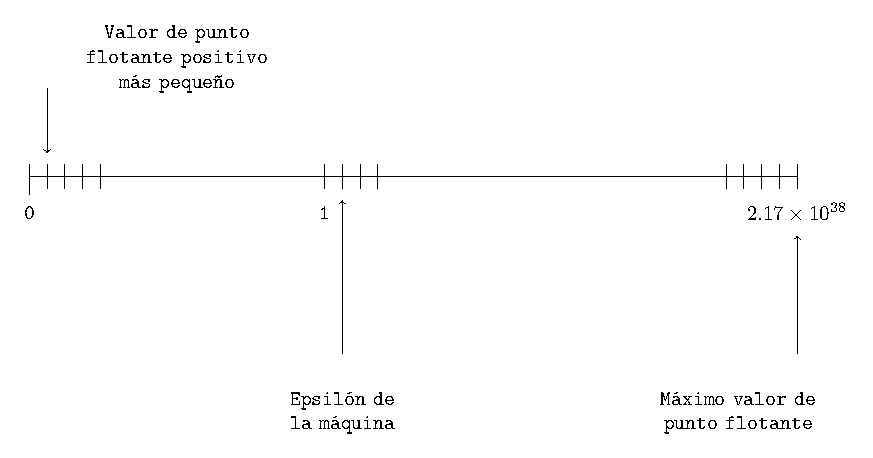
\includegraphics[scale=0.75]{Imagenes/epsilonmaquina.eps}
\end{figure}
\end{frame}
\begin{frame}[fragile]
\frametitle{Pensemos cómo calcular el épsilon relativo}
Una manera sencilla de calcular el épsilon relativo del equipo que estamos usando, es reducir a la mitad un intervalo inicial, hasta cierto punto.
\\
\bigskip
\pause
Dividimos la unidad a la mitad,  \pause luego volvemos a dividir a la mitad.
\end{frame}
\begin{frame}
\frametitle{Pensemos cómo calcular el épsilon relativo}
\begin{figure}
	\begin{tikzpicture}
		\only<1>{\node (Label1) at (6, 1.5) {Tomamos el valor de $1$};}

		\draw (0, 0) rectangle (6, 0.5);
		\draw [<->] (0, -2) -- (6, -2);
		\draw (0, -1.9) -- (0, -2.1);
		\draw (6, -1.9) -- (6, -2.1);
		\draw [color=red] (5, -1.7) node {$1$};
			
		\pause
		
		\only<2>{\node (Label2) at (5, 1.5) {Dividimos a la mitad esta unidad};}
		
		\draw (0, -0.1) rectangle (3, -0.6);
		\draw [dashed] (3,-0.6) -- (3, -2.4);
		\draw [<->] (0, -2.4) -- (3, -2.4);
		\draw [color=red] (2.7, -1.7) node {$\frac{1}{2}$};
		
		\pause

		\only<3>{\node (Label2) at (5, 1.5) {Nuevamente dividimos a la mitad};}

		\draw (0, -0.7) rectangle (1.5, -1.2);
		\draw [dashed] (1.5, -1.2) -- (1.5, -2.8);
		\draw [<->] (0, -2.8) -- (1.5, -2.8);
		\draw [color=red] (1.3, -1.7) node {$\frac{1}{4}$};
		
		\pause

		\only<4>{\node (Label3) at (5, 1.5) {Volvemos a dividir a la mitad};}

		\draw (0, -1.3) rectangle (0.75, -1.8);
		\draw [dashed] (0.75, -1.8) -- (0.75, -3.2);	
		\draw [<->] (0, -3.2) -- (0.75, -3.2);
		\draw [color=red] (0.5, -3.5) node {$\frac{1}{8}$};

		\pause
		
		\only<5>{\node (Label4) at (5, 1.5) {Seguimos dividiendo a la mitad ...};}
	\end{tikzpicture}
\end{figure}
\end{frame}
\begin{frame}
\frametitle{Pasando al código}
Una vez que nos hemos hecho a la idea del procedimiento a seguir, \pause ya podemos proponer una serie de pasos para obtener el valor del \emph{épsilon relativo de la máquina}.
\end{frame}
\begin{frame}[fragile]
\frametitle{Calculemos el épsilon con \python}
\begin{lstlisting}[caption=Código para el épsilon]
t = 1.0

while 1 + t != 1: |\pause|
  eps = t |\pause|
  t = t/2 |\pause|

print('El epsilon de la maquina es: {0:}'.format(eps))
\end{lstlisting}
\end{frame}
\begin{frame}
\frametitle{¿Cómo obtener los valores mínimo y máximo?}
Por curiosidad podemos revisar cuáles son los números más pequeño y más grande para los tipos de datos entero y de punto flotante que podemos representar en una computadora.
\\
\bigskip
\pause
Al igual que en el ejemplo anterior, ocupar inicialmente un bucle sería buena idea, pero veamos algunas funciones útiles en \python.
\end{frame}
\begin{frame}[allowframebreaks, fragile]
\frametitle{Usando una librería y funciones}
\begin{lstlisting}[caption=Obteniendo valores mínimo y máximo]
import sys

i = sys.maxsize
print(i)

f1 = sys.float_info.max
print(f1)

f2 = sys.float_info.min
print(f2)

eps2 = sys.float_info.epsilon
print(eps2)
\end{lstlisting}
\end{frame}

\section{Punto flotante}
\frame{\tableofcontents[currentsection, hideothersubsections]}
\subsection{Introducción}

\begin{frame}
\frametitle{Introducción}
La aritmética que se realiza en una computadora es distinta a la aritmética que hemos aprendido de los cursos de álgebra o cálculo.
\end{frame}
\begin{frame}
\frametitle{Introducción}
Pensaríamos que siempre serían verdaderas las siguientes operaciones:
\pause
\begin{itemize}
\item[\ding{213}] $2 + 2 = 4$
\item[\ding{213}] $4 * 4 = 16$
\item[\ding{213}] $(\sqrt{3})^{2} = 3$
\end{itemize}
Sin embargo, la tercera  operación no siempre se da como la conocemos.
\end{frame}
\begin{frame}
\frametitle{Introducción}
En nuestro mundo matemático se permiten y se manejan  números expresados con una cantidad infinita de cifras.
\end{frame}
\begin{frame}
\frametitle{Introducción}
Sin embargo, en el mundo computacional, cada número representable tiene sólo un número finito de cifras. Esto significa que sólo los números enteros y algunos números racionales se pueden presentar con exactitud. 
\end{frame}
\begin{frame}
\frametitle{Introducción}
Puesto que el número $\sqrt{3}$ no es racional, la computadora le da una representación aproximada, cuyo cuadrado no es $3$, aunque si lo bastante cercano a $3$ para que sea aceptable en la mayor parte de las situaciones.
\end{frame}

\subsection{Números de punto flotante}

\begin{frame}
\frametitle{Representación de punto flotante}
Todos los números deben ser almacenados en la computadora de tal manera que las operaciones aritméticas puedan ejecutarse  con estos números.
\\
\bigskip
\pause
La mayoría de las computadoras tiene dos maneras de guardar estos números:
\setbeamercolor{item projected}{bg=ao,fg=white}
\setbeamertemplate{enumerate items}{%
\usebeamercolor[bg]{item projected}%
\raisebox{1.5pt}{\colorbox{bg}{\color{fg}\footnotesize\insertenumlabel}}%
}
\begin{enumerate}[<+->]
\item Formato de enteros.
\item Formato de punto flotante.
\end{enumerate}
\end{frame}
\begin{frame}
\frametitle{Representación de enteros}
Los número enteros son relativamente directos, en donde debemos de considerar el intervalo donde se puede representar.
\\
\bigskip
\pause
El formato punto flotante es una forma más general permitiendo almacenar números que no son enteros, revisaremos el formato estándar de representación.
\end{frame}
\begin{frame}
\frametitle{Punto flotante para decimales}
Consideremos un número $x$ distinto de cero, escrito en el sistema decimal de manera única como:
\pause
\begin{align*}
x =  \sigma \cdot \overline{x} \cdot 10^{e}
\end{align*}
\pause
donde: 
\begin{itemize}[<+->]
\item[\ding{212}] El \textcolor{lava}{signo} es $\sigma= \pm 1$,
\item[\ding{212}] El \textcolor{cadmiumgreen}{exponente} $e$ es un entero.
\item[\ding{212}] La \textcolor{darkmagenta}{mantisa} es tal que $ 1 \leq \overline{x} \leq 10$.
\end{itemize}
\end{frame}
\begin{frame}
\frametitle{Ejemplo de representación}
Consideremos el número:
\begin{align*}
123.45 = + 1 \cdot (1.2345) \cdot 10^{2}
\end{align*}
\pause
Entonces:
\begin{itemize}[<+->]
\item[\ding{212}] El \textcolor{lava}{signo} es $\sigma = +1$
\item[\ding{212}] El \textcolor{cadmiumgreen}{exponente} es $e = 2$
\item[\ding{212}] La \textcolor{darkmagenta}{mantisa} es $\overline{x} =1.2345$
\end{itemize}
\end{frame}
\begin{frame}
\frametitle{Punto flotante en binario}
El sistema binario representa los números como una suma de múltiplos enteros de potencias de $2$.
\\
\bigskip
\pause
La base del sistema binario son los dígitos $0$ y $1$.
\end{frame}
\begin{frame}
\frametitle{Ejemplo de representación}
El siguiente número $x$ en binario tiene el valor en el sistema decimal como:
\pause
\begin{eqnarray*}
\begin{aligned}
(1101.11)_{2} &= 1 \cdot 2^{3} + 1 \cdot 2^{2} + 0 \cdot 2^{1} + 1 \cdot 2^{0} + \\
 &+ 1 \cdot 2^{-1} + 1 \cdot 2^{-2} = \\[0.5em] \pause
 &= ?
\end{aligned}
\end{eqnarray*}
\end{frame}
\begin{frame}
\frametitle{Representación de punto flotante en binario}
Consideremos el número $x$ escrito en forma binaria, de manera análoga como en el caso decimal:
\pause
\begin{align*}
x =  \sigma \cdot \overline{x} \cdot 2^{e}
\end{align*}
\pause
donde: 
\begin{itemize}[<+->]
\item[\ding{212}] El \textcolor{lava}{signo} es $\sigma= \pm 1$,
\item[\ding{212}] El \textcolor{cadmiumgreen}{exponente} $e$ es un entero.
\item[\ding{212}] La \textcolor{darkmagenta}{mantisa} es una fracción binaria tal que $ (1)_{2} \leq \overline{x} \leq (10)_{2}$.
\end{itemize}
\end{frame}
\begin{frame}
\frametitle{Ejemplo de un número de punto flotante}
Sea el número:
\pause
\begin{align*}
x = (11011.0111)_{2} = +1 \cdot (1.10110111)_{2} \cdot 2^{4}
\end{align*}
\pause
Entonces:
\pause
\begin{itemize}[<+->]
\item[\ding{212}] El \textcolor{lava}{signo} es $\sigma = +1$
\item[\ding{212}] El \textcolor{cadmiumgreen}{exponente} es $e = 4 = (100)_{2}$
\item[\ding{212}] La \textcolor{darkmagenta}{mantisa} es $\overline{x} = (1.10110111)_{2}$
\end{itemize}
\end{frame}
\begin{frame}
\frametitle{Dos observaciones}
\setbeamercolor{item projected}{bg=buff,fg=byzantine}
\setbeamertemplate{enumerate items}{%
\usebeamercolor[bg]{item projected}%
\raisebox{1.5pt}{\colorbox{bg}{\color{fg}\footnotesize\insertenumlabel}}%
}
\begin{enumerate}[<+->]
\item Para todo número $x \neq 0$, el primer dígito de la izquierda del punto en $\overline{x}$, es siempre $1$.
\item La representación de $x$ también está sujeta al número de dígitos binarios en $\overline{x}$ y en el tamaño del exponente.
\end{enumerate}
\end{frame}

\section{Precisión en punto flotante}
\frame[allowframebreaks]{\tableofcontents[currentsection, hideothersubsections]}
\subsection{Definición de precisión}

\begin{frame}
\frametitle{Definición}
El número permitido de dígitos binarios en $\overline{x}$ se le llama \textcolor{blue}{precisión} de la representación de punto flotante binario.
\end{frame}

\subsection{Estándar IEEE 754}
\begin{frame}
\frametitle{El Estándar IEEE 754}
El estándar IEEE 754 para la aritmética de punto flotante es el formato para números puntos flotante usado en computación.
\\
\bigskip
\pause
Este estándar maneja dos tipos de precisión: \textcolor{lava}{simple} y \textcolor{ao}{doble}.
\end{frame}

\subsection{Precisión simple}

\begin{frame}
\frametitle{Precisión simple}
En este estándar, la representación de \emph{\textcolor{darkblue}{punto flotante de precisión simple}} de un número $x$, tiene una precisión de $24$ dígitos binarios y el exponente está limitado a $-126 \leq e \leq 127$:
\pause
\begin{align*}
x = \sigma \cdot (1.a_{1} \, a_{2} \, \ldots \, a_{22} \, a_{23}) \cdot 2^{e}
\end{align*}
\pause
En binario:
\pause
\begin{align*}
-(1111110)_{2} \leq e \leq (1111111)_{2}
\end{align*}
\end{frame}
\begin{frame}
\frametitle{Posición de los bits}
Este formato usa $4$ bytes ($32$  bits), distribuidos de la siguiente manera:
\pause
\begin{figure}
    \centering
    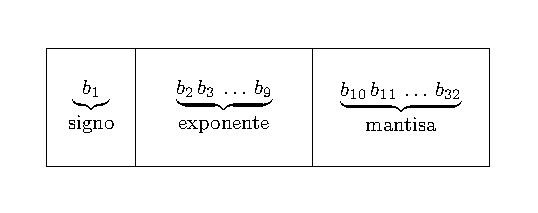
\includegraphics[scale=1.2]{Imagenes/precision_simple.eps}
\end{figure}
\end{frame}
\begin{frame}
\frametitle{Posición de los bits}
\begin{figure}
    \centering
    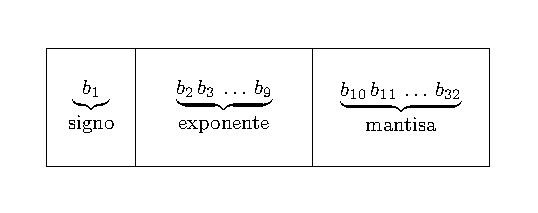
\includegraphics[scale=1.2]{Imagenes/precision_simple.eps}
\end{figure}
\begin{itemize}
\item[\ding{212}] El \textcolor{lava}{signo} $\sigma$ se almacena en el bit $b_{1}$, tal que $b_{1} = 0$ para $\sigma = +1$ y $b_{1} = 1$ para $\sigma = -1$
\end{itemize}
\end{frame}
\begin{frame}
\frametitle{Posición de los bits}
\begin{figure}
    \centering
    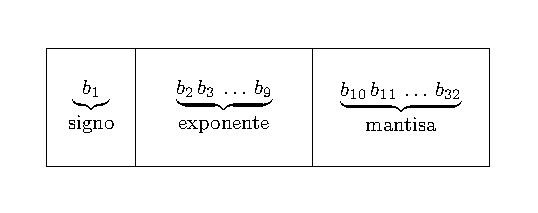
\includegraphics[scale=1.2]{Imagenes/precision_simple.eps}
\end{figure}
\begin{itemize}[<+->]
\item[\ding{212}] Se define $E = e + 127$ como el valor del \textcolor{cadmiumgreen}{exponente} desplazado $127$ lugares.
\item[\ding{212}] Se almacena el entero binario positivo $E$ en los bits $b_{2}$ a $b_{9}$
\end{itemize}
\end{frame}
\begin{frame}
\frametitle{Posición de los bits}
\begin{figure}
    \centering
    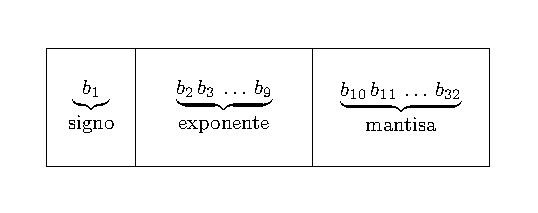
\includegraphics[scale=1.2]{Imagenes/precision_simple.eps}
\end{figure}
\begin{itemize}
\item[\ding{212}] El número binario $a_{1} \, a_{2} \ldots a_{23}$ se almacena en los bits $b_{10}$ a $b_{32}$
\end{itemize}
\end{frame}
\begin{frame}
\frametitle{Observaciones al formato}
El primer dígito binario $1$ de $\overline{x}$ no es guardado en la representación de punto flotante cuando el número se almacena en memoria, \pause pero éste dígito se agrega en $\overline{x}$ cuando el número de punto flotante es llamado de la memoria para ejecutar alguna operación aritmética.
\end{frame}
\begin{frame}
\frametitle{Observaciones al formato}
Se requiere de una representación especial del número $x = 0$, se almacena como:
\begin{itemize}
\item[\ding{212}] $\sigma = 0$
\item[\ding{212}] $\text{exponente} = 0$
\item[\ding{212}] $b_{1} \, b_{2} \, \ldots \, b_{32} = (00 \ldots 0)_{2}$
\end{itemize}
\end{frame}
\begin{frame}
\frametitle{Observaciones al formato}
En precisión simple, el número $1$ se representa por:
\pause
\begin{align*}
1.00000000000000000000000
\end{align*}
\pause
El siguiente número binario más grande es:
\pause
\begin{align*}
1.00000000000000000000001
\end{align*}
siendo $1$ el dígito binario en la posición $23$ en la parte derecha del punto.
\end{frame}
\begin{frame}
\frametitle{Observaciones al formato}
El épsilon de la máquina es $2^{-23}$, entonces tenemos que:
\pause
\begin{align*}
2^{-23} \simeq \num{1.19d-7}
\end{align*}
\pause
Por lo que con el formato de precisión simple del estándar IEEE 754, se pueden aproximar $7$ dígitos decimales de un número $x$ cuando se escribe en su formato decimal.
\end{frame}

\subsection{Precisión doble}

\begin{frame}
\frametitle{Definición de la precisión doble}
La representación de \emph{\textcolor{darkspringgreen}{punto flotante de precisión doble}} del estándar IEEE 754 de un número $x$, tiene una precisión de $53$ dígitos binarios, y el exponente está limitado a $-1022 \leq e \leq 1023$.
\pause
\begin{align*}
x = \sigma \cdot (1.a_{1} \, a_{2} \, \ldots \, a_{51} \, a_{52}) \cdot 2^{e}
\end{align*}
\end{frame}
\begin{frame}
\frametitle{Posición de los bits}
La precisión doble utiliza $8$ bytes ($64$ bits) y los números se almacenan de la siguiente forma::
\pause
\begin{figure}
    \centering
    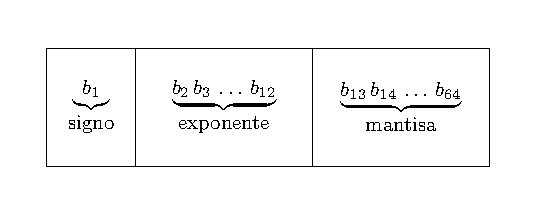
\includegraphics[scale=1.2]{Imagenes/precision_doble.eps}
\end{figure}
\vspace*{-1cm}
Los bits son guardados de manera análoga a la precisión simple, pero con $E = e + 1023$
\end{frame}
\begin{frame}
\frametitle{Observaciones a la precisión doble}
El épsilon de la máquina en precisión doble es:
\pause
\begin{align*}
2^{-52} \simeq \num{2.22d-16}
\end{align*}
\pause
Con el formato de precisión doble del estándar IEEE 754 se puede utilizar para guardar aproximadamente 16 dígitos de un número $x$.
\end{frame}

\subsection*{Casos especiales}

\begin{frame}
\frametitle{Casos especiales del estándar IEEE 754}
Veamos algunos casos especiales de combinaciones entre el signo $(-1)^{s}$, el exponente $e$ y la mantisa $f$:
\pause
\begin{table}
\fontsize{10}{10}\selectfont
\begin{tabular}{l c c}
\hline
Nombre del número & Valores de $\sigma$, $e$, $f$ & Valor \\ \hline
Normal & $0 < e < 255$ & $(-1)^{s} \times 2^{e-127} \times 1.f$ \\ \hline
Subnormal & $e = 0, f \neq 0$ & $(-1)^{s} \times 2^{e-126} \times 0.f$ \\ \hline
Signo cero $(\pm 0)$ & $e = 0, f = 0$ & $(-1)^{s} \times 0.0$ \\ \hline
$+ \infty$ & $s = 0, e=255, f = 0$ & \textbf{\texttt{+INF}} \\ \hline
$- \infty$ & $s = 1, e=255, f = 0$ & \textbf{\texttt{-INF}} \\ \hline
Not a number & $s = u, e=255, f \neq 0$ & \textbf{\texttt{NaN}} \\ \hline
\end{tabular}
\end{table}
\end{frame}
\begin{frame}
\frametitle{Números normales}
Los números normales tienen un valor entre $0 < e < 255$, y con ellos la convención es suponer que el primer bit de la mantisa es un $1$.
\\
\bigskip
\pause
De modo que sólo se almacena la parte fraccional $f$ después del punto binario. 
\end{frame}
\begin{frame}
\frametitle{Valores $\pm \: \text{INF}$ y $NaN$ }
Nótese que los valores $\pm \: \text{INF}$ y $\text{NaN}$ no son números en el sentido matemático, es decir, son objetos que pueden ser manipulados o utilizados en cálculos para tomar límites.
\\
\bigskip
\pause
Más bien, son señales para la computadora y para el usuario de que algo ha ido mal y que el cálculo probablemente debería detenerse hasta resolver las cosas.
\end{frame}
\begin{frame}
\frametitle{Los valores $\pm 0$}
En contraste, el valor $-0$ se puede utilizar en un cálculo sin problemas.
\\
\bigskip
\pause
Algunos lenguajes pueden establecer variables no asignadas como $-0$ como una pista de que aún no se han asignado, pero no es lo más conveniente.
\end{frame}
\begin{frame}
\frametitle{Precisión relativa en punto flotante}
Debido a que la incertidumbre (error) está presente sólo en la mantisa y no en el exponente, las representaciones IEEE aseguran que todos los números normales de punto flotante tengan la misma precisión relativa.
\end{frame}
\begin{frame}
\frametitle{El bit fantasma}
Debido a que el primer bit se supone que es $1$, no tiene que ser almacenado, y los diseñadores de computadoras sólo necesitan recordar que hay un \emph{bit fantasma} allí para obtener un poco más de precisión.
\end{frame}
\begin{frame}
\frametitle{El primer bit}
Durante el procesamiento de números en un cálculo, el primer bit de un resultado intermedio puede llegar a ser cero, pero éste se cambia antes de que se almacene el número final.
\\
\bigskip
\pause
Para repetir, en los casos normales, la mantisa real ($1.f$ en notación binaria) contiene un $1$ implícito que precede al punto binario.
\end{frame}
\begin{frame}
\frametitle{El número de sesgo}
Con el fin de garantizar que el exponente $e$ almacenado sea siempre positivo, se agrega un número fijo llamado \textoazul{sesgo} al exponente real $p$, antes de que se almacene como exponente $e$.
\\
\bigskip
\pause
El exponente real, que puede ser negativo, es:
\pause
\begin{equation}
p = e - \text{sesgo}
\label{eq:ecuacion_01_03b}
\end{equation}
\end{frame}




% \section{Números en la computadora}
% \frame[allowframebreaks]{\tableofcontents[currentsection, hideothersubsections]}
% \subsection{Los números en la computadora}

% \begin{frame}
% \frametitle{Los números en la computadora}
% Las computadoras son herramientas muy poderosas, pero tienen un alcance finito.
% \\
% \bigskip
% \pause
% Un problema que se presenta en el diseño de computadora es cómo representar un número arbitrario usando una cantidad finita de espacio de memoria y cómo tratar con las limitaciones que surgen de esta representación.
% \end{frame}
% \begin{frame}
% \frametitle{Los números en la computadora}
% Como consecuencia de que las memorias de la computadora se basan en un estado de magnetización o electrónico de un giro que apunta hacia arriba o hacia abajo, las unidades más elementales de memoria de la computadora son los dos enteros binarios (bits) $0$ y $1$.
% \end{frame}
% \begin{frame}
% \frametitle{Los números en la computadora}
% Esto significa que la forma en que se almacenan los números en memoria, es como cadenas largas de ceros y unos, es decir, de modo binario.
% \end{frame}

% \subsection{Rango de operación}

% \begin{frame}
% \frametitle{Rango de representación}
% De esta manera: $N$ bits almacena números enteros en el rango $[0, 2^{N}]$, pero debido a que el signo del número entero está representado por el primer bit (un bit cero para números positivos), el rango real disminuye a:
% \pause
% \begin{align*}
% \big[ 0, 2^{N- 1} \big]
% \end{align*}
% \end{frame}
% \begin{frame}
% \frametitle{Otras bases de operación}
% La representación binaria de números a través de ceros y unos, funciona y opera bien para las computadoras, pero no para los usuarios.
% \\
% \bigskip
% \pause
% Es por ello que las cadenas binarias se convierten en números octal, decimal o hexadecimal antes de que los resultados se presenten a los usuarios.
% \end{frame}
% \begin{frame}
% \frametitle{Otras bases de operación}
% Los números octales y hexadecimales son también oportunos porque en la conversión no se pierde precisión.
% \\
% \bigskip
% \pause
% Pero no todo queda bien ya que nuestras reglas decimales de aritmética no funcionan para ellos.
% \end{frame}

% \subsection{Aritmética binaria}

% \begin{frame}
% \frametitle{Desventaja de la aritmética binaria}
% La conversión a números decimales hace que los números sean más fáciles de trabajar, pero a menos que el número sea una potencia de $2$, el proceso conduce a una disminución en la precisión.
% \end{frame}

% \begin{frame}
% \frametitle{Longitud de palabra}
% Una descripción de un sistema informático particular indica normalmente la \emph{longitud de la palabra}, siendo el número de bits utilizados para almacenar un número.
% \\
% \bigskip
% \pause
% La longitud se expresa en bytes, donde:
% \pause
% \begin{align*}
% 1 \text{ byte} \equiv 1 \text{ B} \equiv 8 \: \si{\bit}
% \end{align*}
% \end{frame}

% \subsection{Unidades de medida}

% \begin{frame}
% \frametitle{Unidades de medida}
% Tanto la memoria como el almacenamiento se mide en bytes, kilobytes, megabytes, gigabytes, terabytes y petabytes $(\num{10d15})$.
% \\
% \bigskip
% \pause
% No debemos de confundirnos al elegir las unidades de medida, ya que el prefijo \emph{kilo}, no siempre equivale a $1000$
% \pause
% \begin{align*}
% 1 \: \si{\kilo} =   1 \: \si{\kilo \byte} = \num{2d10} \, \si{\byte} = 1024 \: \si{byte}
% \end{align*}
% \end{frame}
% \begin{frame}
% \frametitle{Unidades de medida}
% La memoria de las primeras computadoras usaban palabras de $8$ bits, esto implicaba que el mayor entero era $2^{7} = 128$, ($7$ debido a $1$ bit para el signo).
% \end{frame}

\subsection{Overflow y underflow}

\begin{frame}
\frametitle{Overflow y underflow}
Si queríamos almacenar un número más grande, tanto el hardware como el software se diseñaban para generar un \textoazul{desbordamiento (overflow)}.
\\
\bigskip
\pause
Se genera un \textoazul{underflow} cuando queremos representar un número más pequeño del que se puede en el equipo.
\end{frame}
\begin{frame}
\frametitle{Errores de almacenamiento: overflow}
Los números de máquina tienen un máximo y un mínimo.
\\
\bigskip
Si se supera el máximo, se produce una condición de error conocida como \textoazul{desbordamiento -overflow-}.
\begin{figure}
\centering
\includestandalone[scale=0.75]{Figuras/over_underflow}
\end{figure}
\end{frame}
\begin{frame}
\frametitle{Errores de almacenamiento: underflow}
\begin{figure}
\centering
\includestandalone[scale=0.75]{Figuras/over_underflow}
\end{figure}
Si se cae por debajo del mínimo, se produce una condición de error conocida como \textoazul{subflujo -underflow-}.
\end{frame}
\begin{frame}
\frametitle{Manejo del overflow y del underflow}
En este último caso, el software y el hardware se pueden configurar para que los overflow se pongan a cero sin que se le avise al usuario.
\\
\bigskip
\pause
En contraste, los overflow suelen detener la ejecución.
\end{frame}

\section{Fuentes de errores}
\frame{\tableofcontents[currentsection, hideothersubsections]}
\subsection{Algo de teoría de errores}

\begin{frame}
\frametitle{Hablando de errores}
Para entender el por qué los errores deben ser motivo de preocupación, imaginemos un programa con el siguiente flujo lógico:
\pause
\begin{equation}
\text{Inicio } \rightarrow U_{1} \rightarrow U_{2} \rightarrow \ldots \rightarrow U_{n} \rightarrow \text{ Fin} 
\label{eq:ecuacion_02_01}
\end{equation}
\end{frame}
\begin{frame}
\frametitle{Hablando de errores}
\begin{equation*}
\text{Inicio } \rightarrow U_{1} \rightarrow U_{2} \rightarrow \ldots \rightarrow U_{n} \rightarrow \text{ Fin} 
\end{equation*}
Donde cada unidad $U$ puede ser una declaración de una tarea o un paso.
\\
\bigskip
\pause
Si cada unidad tiene probabilidad $p$ de ser correcta, entonces la probabilidad conjunta $P$ de que todo el programa sea correcto es $P = p^{n}$.
\\
\end{frame}
\begin{frame}
\frametitle{Hablando de errores}
Digamos que tenemos un programa de tamaño mediano con $n = 1000$ pasos y que la probabilidad de que cada paso sea correcto es casi uno, $p \simeq 0.9993$.
\end{frame}
\begin{frame}
\frametitle{Hablando de errores}
Esto significa que terminaremos con $P \simeq \frac{1}{2}$, es decir, la respuesta final es tan probablemente correcta como equivocada.
\end{frame}
\begin{frame}
\frametitle{Hagamos una sencilla suma}
El resultado de la siguiente suma es muy sencillo:
\pause
\begin{align*}
1.0 + 0.0000001
\end{align*}
\pause
Repitamos esta suma $1000000$ veces, ya conocemos de antemano su resultado. \pause Hagamos un código en \python.
\end{frame}
\begin{frame}[fragile]
\frametitle{Sumando valores}
\begin{lstlisting}[caption=Sumando en un ciclo]
suma = 1.0

for in in range(1, 1000001):
    suma += 0.0000001

print('La suma es: {0:}'.format(suma))
\end{lstlisting}
Calcula el error relativo.
\end{frame}
\begin{frame}
\frametitle{¿En qué nos equivocamos?}
El error relativo es:
\begin{align*}
5.307875351366998e-11
\end{align*}
\pause
Vayamos por partes para revisar dónde se origina el error:
\\
\bigskip
\pause
Para ello, tenemos que ocupar la representación en binario de los dos sumandos: $1.0$ y $0.00001$.
\end{frame}
\begin{frame}
\frametitle{Los sumandos}
En binario tenemos que:
\pause
\begin{align*}
{}&(1)_{10} = (0.1000 0000 0000 0000 0000 0000 0000 0000 0000) \times 2^{1} \\
{}&(0.00001)_{10} = (0.1010011111000101) \times 2^{-32}
\end{align*}
\pause
Ahora sumemos estos dos números.
\end{frame}
\begin{frame}
\frametitle{El valor luego de la suma}
Así llegamos al valor:
\pause
\begin{eqnarray*}
{}&(1)_{10} + (0.00001)_{10} \simeq \\[0.5em] \pause
&\simeq (0.10000000000000001010011111000101) \times 2^{1}
\end{eqnarray*}
\pause
Cuya representación en decimal es:
\pause
\begin{align*}
1.00000000000000005551115123125782
\end{align*}
\end{frame}
\begin{frame}
\frametitle{Error acumulado}
Entonces cada vez que sumemos $0.0000001$ a $1$ se agrega un error de $\num{5.5511d-17}$, \pause y si hacemos la operación un millón veces, \pause encontramos el valor del error relativo que nos devuelve la suma. 
\end{frame}
\begin{frame}
\frametitle{Ajustando el código}
Nuestro trabajo será siempre minimizar los errores como en el caso de la suma anterior.
\\
\bigskip
\pause
En ese mismo ejemplo haremos un ajuste en el código y veremos el resultado obtenido.
\end{frame}
\begin{frame}[allowframebreaks, fragile]
\frametitle{Un ajuste al código}
\begin{lstlisting}[caption=Una agrupación en la suma]
suma = 1.0

for i in range(1, 1001):
    total = 0.0
    for j in range(1, 1001):
        total += 0.0000001
    
    suma = suma + total

print('La suma es: {0:}'.format(suma))
print()
print('El error relativo es: {0:}'.format(error_relativo(1.1, suma)))
\end{lstlisting}
\end{frame}
\begin{frame}
\frametitle{Resultado luego del ajuste al código}
El error realtivo es: $1.00929e-14$, vemos que disminuye $3$ órdenes de magnitud con respecto al primer código.
\\
\bigskip
\pause
La estrategia de agrupar las sumas favoreció para que el error relativo disminuyera.
\end{frame}

\begin{frame}
\frametitle{Ejercicio a cuenta}
\textbf{Ejercicio a cuenta: } El número $\ln \, 2$ se puede calcular de la serie:
\begin{align*}
\ln 2 = 1 - \dfrac{1}{2} + \dfrac{1}{3} -\dfrac{1}{4} + \ldots
\end{align*}
Se sabe del análisis que esta serie converge y que la magnitud del error en cualquier suma parcial es menor que la magnitud del primer término despreciado.
\end{frame}
\begin{frame}
\frametitle{Ejercicio a cuenta}
Estima el número de términos que se requerirían para calcular $\ln 2$ con $10$ decimales.
\end{frame}
\begin{frame}
\frametitle{Ejercicio a cuenta}
\textbf{Ejercicio a cuenta: } El 25 de febrero de 1991, durante la guerra del Golfo, una batería de misiles Patriot americanos en Dharan (Arabia Saudita) no lograron interceptar un misil Scud iraquí. Murieron 28 soldados americanos.
\end{frame}
\begin{frame}
\frametitle{Ejercicio a cuenta}
La causa: los errores numéricos por utilizar truncado en lugar de redondeo en el sistema que calcula el momento exacto en que debe ser lanzado el misil.
\\
\bigskip
\pause
Las computadoras de los Patriot que han de seguir la trayectoria del misil Scud, la predicen punto a punto en función de su velocidad conocida y del momento en que fue detectado por última vez en el radar.
\end{frame}
\begin{frame}
\frametitle{Ejercicio a cuenta}
La velocidad es un número real. El tiempo es una magnitud real pero el sistema la calculaba mediante un reloj interno que contaba décimas de segundo, por lo que representaban el tiempo como una variable entera.
\\
\bigskip
\pause
Cuanto más tiempo lleva el sistema funcionando más grande es el entero que representa el tiempo.
\end{frame}
\begin{frame}
\frametitle{Ejercicio a cuenta}
Las computadoras del Patriot almacenan los números reales representados en punto flotante con una mantisa de $24$ bits.
\\
\bigskip
\pause
Para convertir el tiempo entero en un número real se multiplica éste por $1/10$, y se trunca el resultado (en lugar de redondearlo). El número $1/10$ se almacenaba truncado a $24$ bits.
\end{frame}
\begin{frame}
\frametitle{Ejercicio a cuenta}
El pequeño error debido al truncado, se hace grande cuando se multiplica por un número (entero) grande, y puede conducir a un error significativo.
\\
\bigskip
La batería de los Patriot llevaba en funcionamiento más de $100$ horas, por lo que el tiempo entero era un número muy grande y el número real resultante tendrá un error cercano a $0.34$ segundos. \pause Explica a detalle qué fue lo que ocurrió.
\end{frame}
\begin{frame}
\frametitle{Entrega de los ejercicios a cuenta}
Estos ejercicios a cuenta, se deberán de entregar a más tardar para el día domingo a las $12$ del día vía Moodle.
\\
\bigskip
Recuerda que puedes usar una notebook de Jupyter o archivo *.py (que deberán estar en un *.zip)
\end{frame}
\end{document}